\section{Experiments}
\label{sec:experiments}

\providecommand{\Kdef}{16}
\providecommand{\needsnum}[1]{\textcolor{red}{\textbf{[NEED: #1]}}}

We organize the evaluation around interventions rather than datasets, so that each claim has a matching experiment. The method separates three mechanisms, namely the witness gate $g$ (exposure), the learned magnitude $\lambda_s$ (strength), and the direction $f_{\rm mat}$. The experiments isolate them in turn.
\begin{itemize}\itemsep2pt
  \item[\textbf{RQ1}] \emph{Exposure.} Does the witness expose the material force when a feasible lower-risk maneuver exists and suppress it otherwise? (\S\ref{sec:exp_primary_delayed})
  \item[\textbf{RQ2}] \emph{Witness validity.} Does witness feasibility predict the safety-relevant properties of the executed motion, despite not prescribing its path? (\S\ref{sec:exp_rellis_dyn})
  \item[\textbf{RQ3}] \emph{Force efficacy.} Does the material channel change behavior when its learned magnitude is large? (\S\ref{sec:exp_dfc})
  \item[\textbf{RQ4}] \emph{Adaptation.} What do the context-conditioned magnitude and CVaR add, relative to a tuned constant and expected-cost training? (\S\ref{sec:exp_adapt})
  \item[\textbf{RQ5}] \emph{Robustness.} How sensitive are these effects to perception quality, candidate count $K$, and training-map diversity? (\S\ref{sec:exp_interpretation})
\end{itemize}
End-to-end planner comparisons (\S\ref{sec:exp_e2e}) are evaluation.
 
\subsection{Setup, metrics, and domains}
\label{sec:exp_setup}

\paragraph{Regimes.} All domains share \textbf{R1} (a feasible lower-risk alternative exists), \textbf{R2} (the lower-risk-looking direction is blocked or dynamically unsafe), and \textbf{R3} (risk-neutral; the material-aware policy should preserve geometry-only behavior). RELLIS-Dyn extends R1/R2 from space to time through eight event types (Appendix~\ref{app:rellis_dyn}). The head-to-head diagnostic is \emph{delayed required escape}, in which the maneuver is blocked before $t_{\rm escape}$ and necessary after.

\paragraph{Metrics.} Selectivity is measured on the \emph{gated material force} $F_{\rm mat}^{\rm exec}=g\,\lambda_s f_{\rm mat}$ (the hazard force is excluded so it cannot contaminate the reading), and is defined by
\begin{equation}
\mathrm{CAR}=\Pr[\langle F_{\rm mat}^{\rm exec},d_{\rm safe}\rangle{>}\epsilon\mid \mathrm{R1}],\;
\mathrm{FAR}=\Pr[\,|P_\perp F_{\rm mat}^{\rm exec}|{>}\epsilon\mid \mathrm{R2}],\;
\mathrm{SR}=\frac{\mathbb E[\,|P_\perp F_{\rm mat}^{\rm exec}|\mid \mathrm{R1}]}
                 {\mathbb E[\,|P_\perp F_{\rm mat}^{\rm exec}|\mid \mathrm{R2}]}.
\end{equation}
Temporal metrics are \emph{false pre-activation} (lateral force before $t_{\rm escape}$), \emph{suppress rate} ($1-$false pre-activation), \emph{reaction delay}, and post-event \emph{violation CVaR} (the primary tail metric). We use $K{=}\Kdef$ sampled primitives unless noted.

\subsection{(RQ1) Exposure, or how the witness controls \emph{when} the force acts}
\label{sec:exp_primary_delayed}

\paragraph{The gate, not the coefficient, controls exposure.}
Holding the trained model fixed and toggling only the gate, soft-force exposure collapses across all three regimes (Table~\ref{tab:gate_toggle}). On this delayed-escape checkpoint the learned $\lambda_s$ is small ($\approx0.06$), so end-to-end success and violation CVaR barely move when the gate is toggled. The gate cleanly decides \emph{whether} the material force is exposed, while its \emph{magnitude} here is small. Delayed escape is therefore \emph{diagnostic for exposure timing}, not a demonstration that the soft force itself drives the outcome that is RQ3.

\begin{table}[t]
\centering
\caption{\textbf{Gate toggle} (same trained model, gate forced on vs.\ off;
$100$ paired episodes on identical seeds and events). ``Exposure'' is the
fraction of control steps at which the material force reaches the executed
field, so gate-off is $1.000$ by construction. The witness gate removes
$91$--$94\%$ of exposure across all three regimes, isolating \emph{when} the
channel acts from \emph{how strongly} it acts. Outcome metrics are essentially
unchanged here because the learned $\lambda_s\!\approx\!0.06$ on this
checkpoint, so this benchmark is diagnostic for exposure timing rather than a
demonstration that the soft force drives the outcome (that is RQ3). The two
arms also follow the same path (Fig.~\ref{fig:rq1}F). Full CIs in
App.~\ref{app:gate_toggle}.}
\label{tab:gate_toggle}
\small
\setlength{\tabcolsep}{6pt}\renewcommand{\arraystretch}{1.1}
\begin{tabular}{lccc}
\toprule
Regime & Exposure (gate on) & Exposure (gate off) & Reduction \\
\midrule
R1 & $0.094$ & $1.000$ & $0.906$ \\
R2 & $0.061$ & $1.000$ & $0.939$ \\
R3 & $0.076$ & $1.000$ & $0.924$ \\
\bottomrule
\end{tabular}
\end{table}

\paragraph{Activation is sparse and time-concentrated.}
Across the delayed-escape episodes the gate is active on only $7.77\%$ of steps (at $K{=}\Kdef$) and fires at least once in $76/100$ episodes, concentrating after the escape becomes feasible (Table~\ref{tab:activation_profile}; App.~Fig.~\ref{fig:rq1} shows the gate decisions in a single rollout, together with the evidence that the gate changes exposure without changing the executed path). This is the intended signature of a conditional mechanism rather than an always-on potential. The gate is recomputed frame-wise with no hysteresis, so it can flicker, and $33.8\%$ of activation periods last a single step (\S\ref{sec:exp_interpretation}).

\begin{table}[t]
\centering
\caption{\textbf{Gate activation profile} (delayed-required escape, $100$
episodes, $K{=}\Kdef$ sampled primitives). Fraction of control steps at which
the gate admits the material force, by episode phase and regime. Activation
rises sharply once the escape becomes feasible, which is the intended signature
of a conditional mechanism. The final column reports flicker, meaning the fraction of
activation periods lasting a single step, a consequence of recomputing the gate
frame-wise with no hysteresis. Per-phase detail in
App.~Table~\ref{tab:app_activation}.}
\label{tab:activation_profile}
\small
\setlength{\tabcolsep}{8pt}\renewcommand{\arraystretch}{1.1}
\begin{tabular}{lcccc}
\toprule
Phase & Pre-event & Blocked & Post-opening & Overall \\
\midrule
Activation rate & $3.61\%$ & $5.70\%$ & $13.39\%$ & $7.77\%$ \\
\bottomrule
\end{tabular}
\end{table}

\paragraph{Head-to-head.}
Table~\ref{tab:delayed_escape} places the full system against reactive, sampling, and learned baselines under an identical per-step BEV patch. The gated, CVaR-trained field suppresses early false activation ($0.950\!\to\!0.380$ vs.\ DWA; paired difference $-0.57$, $95\%$ CI $[-0.67,-0.47]$) while still succeeding after the escape opens ($0.480\!\to\!0.610$; paired difference $+0.13$, $95\%$ CI $[0.03,0.23]$), with zero replans. The fixed-\emph{high}-coefficient field without a gate over-activates (false pre-act $0.990$), which is a gate failure rather than a coefficient success. It is the absence of exposure control, not the coefficient value, that breaks suppression.

\begin{table}[t]
\centering
\caption{\textbf{Delayed-required-escape} head-to-head ($100$ paired episodes).
The nominal route is blocked at $t_{\rm event}$, an alternative becomes feasible
$10$ steps later, and the nominal route is simultaneously sealed, so acting on
the escape is \emph{required} rather than optional. All methods see an identical
per-step BEV patch. False pre-activation is lateral material force applied
before the escape is feasible (lower better), suppression its complement,
success reaching the goal, and violation CVaR the post-event tail metric (lower
better). \emph{Bold marks our method's row, not the best value in each column}. The
geometry-only policy attains a lower false pre-activation ($0.000$) by never
activating at all, at $0.030$ success.
$^\dagger$Low CVaR with success ${<}0.21$ reflects low exposure from
getting stuck, not safe behaviour. CIs in
App.~Table~\ref{tab:app_delayed_escape_ci}; the expected-cost versus CVaR
comparison is analysed in Fig.~\ref{fig:rq4}.}
\label{tab:delayed_escape}
\small
\setlength{\tabcolsep}{4pt}\renewcommand{\arraystretch}{1.1}
\begin{tabular}{lcccc}
\toprule
Method & False pre-act$\downarrow$ & Suppress$\uparrow$
       & Success$\uparrow$ & Viol.\ CVaR$\downarrow$ \\
\midrule
Geometry-only policy        & $0.000$ & $1.000$ & $0.030$ & $1.894$ \\
Risk-loss-only              & $0.420$ & $0.580$ & $0.040$ & $1.793$ \\
Fixed-coeff (no gate)       & $0.990$ & $0.010$ & $0.030$ & $0.463^\dagger$ \\
Black-box CVaR              & $0.920$ & $0.080$ & $0.200$ & $0.503^\dagger$ \\
DWA semantic                & $0.950$ & $0.050$ & $0.480$ & $0.695$ \\
MPPI semantic               & $0.950$ & $0.050$ & $0.240$ & $0.831$ \\
Material-aware, expected cost & $0.370$ & $0.630$ & $0.620$ & $0.855$ \\
\textbf{Material-aware, gated + CVaR}
  & $\mathbf{0.380}$ & $\mathbf{0.620}$ & $\mathbf{0.610}$ & $\mathbf{0.840}$ \\
\bottomrule
\end{tabular}
\end{table}

\subsection{(RQ2) Witness validity, or evidence rather than a tracked path}
\label{sec:exp_rellis_dyn}

The witness primitive $k^\star$ is a feasibility sensor, so we check whether it predicts the executed motion's safety-relevant properties, \emph{not} whether the path is reproduced (Table~\ref{tab:witness_validity}). Path agreement is deliberately loose, and over all $492$ activations the median direction cosine is $0.717$ (mean $0.705$) and the mean endpoint gap is $4.46$\,m, confirming the field, not $k^\star$, generates motion. Yet in the post-opening phase, where the feasibility signal is least temporally confounded, the executed motion agrees with the witness on clearance $74.3\%$ of the time and disagrees on hard contact only $10.6\%$. Aggregated over the full episode (including the pre-opening phase where the escape is correctly not yet acted on) agreement is naturally lower. Feasibility of the witness thus transfers to the executed trajectory on the dimensions that matter, even though the path is not. App.~Figure~\ref{fig:rq2} draws the logged witness rays against the executed steps and quantifies the separation, for which the median angle between them is $45^\circ$.

\begin{table}[t]
\centering
\caption{\textbf{Witness--execution agreement} ($492$ gate-positive
activations). The witness primitive $k^\star$ is evidence that a lower-risk
motion exists, not a reference the controller tracks, so we test whether it
predicts the executed motion's safety-relevant properties rather than its
geometry. Path rows measure geometric similarity; property rows measure
agreement on clearance, hard contact, and the sign of the predicted risk
improvement. ``Post-opening'' restricts to steps after the escape becomes
feasible, where the signal is least temporally confounded. Path agreement is
deliberately loose while property agreement is high, because the field, not
$k^\star$, generates motion. Geometry in Fig.~\ref{fig:rq2}.}
\label{tab:witness_validity}
\small
\setlength{\tabcolsep}{6pt}\renewcommand{\arraystretch}{1.1}
\begin{tabular}{lcc}
\toprule
 & Post-opening & Full episode \\
\midrule
\multicolumn{3}{l}{\emph{Path agreement}}\\
Direction cosine (median) & $0.727$ & $0.717$ \\
Direction cosine (mean)   & $0.690$ & $0.705$ \\
Endpoint gap (mean, m)    & $4.56$  & $4.46$  \\
\midrule
\multicolumn{3}{l}{\emph{Safety properties}}\\
Clearance agreement   & $74.3\%$ & $55.6\%$ \\
Hard-contact disagreement & $10.6\%$ & n/a \\
Risk-sign agreement   & n/a & $52.9\%$ \\
\bottomrule
\end{tabular}
\end{table}

\paragraph{Spatial and temporal selectivity.}
On RELLIS-3D (2{,}250 BEV episodes, leave-one-sequence-out; full table in App.~\ref{app:rellis_full}) the material-aware field attains the best suppression ratio, $\mathrm{SR}=2.358$ vs.\ $1.292$ for black-box CVaR, with $\mathrm{FAR}=0.114$; black-box CVaR reaches a marginally higher CAR ($0.884$ vs.\ $0.837$) but far worse spatial suppression, so our advantage is on SR and FAR, not CAR. The decisive point is temporal, since that same black-box model, despite $\mathrm{CAR}=0.884$, succeeds on only $0.200$--$0.273$ of temporal episodes (Tables~\ref{tab:delayed_escape},~\ref{tab:rellis_dyn_agg}). \emph{Static selectivity does not predict navigation success}  which is precisely what the witness gate is for.

\subsection{(RQ3) Force efficacy of the material channel on its own axis}
\label{sec:exp_dfc}

To isolate the soft channel we vary only $\lambda_s$ with the hazard coefficient $\lambda_h$ fixed, same checkpoint, gate, and episodes (Table~\ref{tab:one_factor}). Where the material field is informative (DFC2018, dense semantics) the recovered magnitude is large ($\lambda_s$ mean $1.813$, median $2.250$) and enabling it alone reduces cumulative material risk ($10.340\!\to\!10.288$, $95\%$ CI excluding zero) at unchanged $100\%$ success. Where semantics are sparse (RELLIS R1) the magnitude is small and the isolated effect is not significant (CI includes zero). The channel thus contributes when it carries weight and correctly downscales itself when the map is uninformative. App.~Figure~\ref{fig:rq3} shows the per-episode paired distributions behind both rows, on a magnified scale that makes the size of the DFC2018 effect explicit.

\begin{table}[t]
\centering
\caption{\textbf{Isolated soft coefficient} ($\lambda_s$ varied, $\lambda_h$ fixed; 540 paired episode-arms). The material channel is effective where the material field is informative and near-silent where it is not.}
\label{tab:one_factor}
\small
\setlength{\tabcolsep}{6pt}\renewcommand{\arraystretch}{1.1}
\begin{tabular}{lccc}
\toprule
Domain & Recovered $\lambda_s$ (mean/med) & Isolated soft-risk effect & Success \\
\midrule
DFC2018 (dense)    & $1.813 / 2.250$ & $10.340\!\to\!10.288$ (CI excl.\ 0) & $1.000$ \\
RELLIS R1 (sparse) & $0.107 / 0.109$ & $16.764\!\to\!16.763$ (CI incl.\ 0) & $1.000$ \\
\bottomrule
\end{tabular}
\end{table}

\paragraph{End-to-end DFC repair.}
Beyond the isolated coefficient, the full material-aware policy repairs a geometry-only policy on the static semantic map (Table~\ref{tab:dfc_geom_ctx}), raising success $0.867\!\to\!1.000$, catastrophic failure $0.600\!\to\!0.100$, cumulative risk $23.27\!\to\!9.49$, oscillation $-90.7\%$, path length unchanged. Note that this $23.27\!\to\!9.49$ is the \emph{combined} effect of all coefficients and is a different comparison from the isolated $10.340\!\to\!10.288$ above.

\begin{table}[t]
\centering
\caption{\textbf{DFC2018 combined repair} ($300$ paired episodes; dense
semantic map). A geometry-only policy versus the full material-aware policy on
identical episodes, with \emph{all} coefficients active. ``Catastrophic
failure'' is an episode with at least one hard-hazard contact; oscillation is
total absolute heading change along the path, $\sum_t|\Delta\theta_t|$. This is the combined
effect of every channel and is therefore a different comparison from the
one-factor $\lambda_s$ intervention in Table~\ref{tab:one_factor}, where only
the soft coefficient changes and the effect is correspondingly much smaller.}
\label{tab:dfc_geom_ctx}
\scriptsize\setlength{\tabcolsep}{3pt}\renewcommand{\arraystretch}{1.08}
\resizebox{0.72\linewidth}{!}{%
\begin{tabular}{lrrrrrr}
\toprule
Method & Succ.$\uparrow$ & Cat.fail$\downarrow$ & Hard len.$\downarrow$
       & Risk$\downarrow$ & Len.ratio & Osc.$\downarrow$ \\
\midrule
Geometry-only policy & $0.867$ & $0.600$ & $21.106$ & $23.267$ & $1.044$ & $82.212$ \\
\textbf{Material-aware} & $\mathbf{1.000}$ & $\mathbf{0.100}$ & $\mathbf{0.658}$
                 & $\mathbf{9.493}$ & $1.045$ & $\mathbf{7.629}$ \\
\bottomrule
\end{tabular}}
\end{table}

\subsection{(RQ4) Adaptation, or why learn $\lambda_s$ and what CVaR adds}
\label{sec:exp_adapt}

\paragraph{Cross-domain scaling, not within-domain superiority.}
The value of the context-conditioned head is that one model recovers very different magnitudes without retuning, with $\lambda_s\approx0.06$ on RELLIS off-road (delayed-escape checkpoint), $\approx0.11$ on RELLIS R1, versus $\approx1.8$ on DFC (Table~\ref{tab:one_factor}), roughly a $17{\times}$ range across domains. Within a single domain, a well-tuned fixed $\lambda_s$ is competitive; we therefore do not claim the learned coefficient beats a tuned constant per domain, only that it removes the per-domain retuning a fixed value would require. App.~Figure~\ref{fig:rq4} shows the recovered coefficient distributions across the three settings and locates the CVaR tail spatially.

\paragraph{The objective is not what drives suppression.}
Holding architecture and gate fixed and changing only the objective (expected cost vs.\ CVaR), no metric separates the two arms at $95\%$ confidence over $100$ paired episodes, with false pre-activation $0.370$ vs.\ $0.380$ (paired difference $+0.01$, CI $[-0.04,0.06]$), suppression $0.630$ vs.\ $0.620$ (CI $[-0.06,0.04]$), success $0.620$ vs.\ $0.610$ (CI $[-0.05,0.03]$), and violation CVaR $0.855$ vs.\ $0.840$ (CI $[-0.034,0.004]$) (Table~\ref{tab:delayed_escape}; App.~Table~\ref{tab:app_delayed_escape_ci}). The tail-sensitive objective is therefore \emph{not} the source of the suppression behaviour on this benchmark. That is the gate's role, as the gate-toggle intervention in Table~\ref{tab:gate_toggle} shows directly. We report the CVaR objective as the training choice we used, not as a demonstrated contributor to these outcomes.

\subsection{(RQ5) Robustness}
\label{sec:exp_interpretation}

\paragraph{Perception.}
Under a realistic learned semantic predictor (rather than ground truth) in a leakage-free same-episode split, selectivity is essentially preserved (CAR $+0.024$, FAR $+0.009$, SR $+0.129$ vs.\ ground truth). Under deliberately harsher label corruption, degradation is monotone rather than a collapse, but it is substantial, since CAR falls $0.733\!\to\!0.489\!\to\!0.397\!\to\!0.347$ at $0/10/20/30\%$ corruption while FAR falls in step ($0.217\!\to\!0.134$), so the selectivity ratio declines only from $1.864$ to $1.549$ and activation drops from $0.287$ to $0.158$ (Table~\ref{tab:perception}). Tracking the $52{,}113$ decision points matched across all four corruption levels shows the suppression is indiscriminate. Activations that were correct on the clean map survive at rate $0.414$ at $30\%$ corruption, and those that were false survive at $0.446$, a gap of only $0.032$ (Fig.~\ref{fig:rq5}). The failure mode is conservatism, not improved discrimination. Because activation requires risk improvement, clearance, and traversability jointly, an isolated corrupted low-risk patch does not on its own trigger the soft force. This is empirical graceful degradation, not a perception guarantee, since the method does not correct systematically wrong maps online and does not use calibrated uncertainty. We distinguish realistic prediction error (little effect) from adversarial corruption (the degradation curve); $30\%$ corruption is a pessimistic stress test, not a deployment condition.

\begin{table}[t]
\centering
\caption{\textbf{Perception degradation} on RELLIS-3D selectivity
($2{,}250$ episodes, $293$ scenes; frozen clean LOSO heads evaluated on
corrupted semantic labels). Correct-activation rate (CAR) and false-activation
rate (FAR) both fall as labels are corrupted, so the selectivity ratio
$\mathrm{SR}=\mathrm{CAR}/\mathrm{FAR}$ degrades but stays above~$1.5$, so the
controller becomes uniformly more conservative rather than selectively wrong.
Brackets are $95\%$ cluster-bootstrap CIs (episode is the resampling unit).
Full CIs and the learned-predictor split in App.~\ref{app:perception};
decision-level analysis in Fig.~\ref{fig:rq5}.}
\label{tab:perception}
\small
\setlength{\tabcolsep}{5pt}\renewcommand{\arraystretch}{1.1}
\begin{tabular}{lcccc}
\toprule
Label corruption & $0\%$ & $10\%$ & $20\%$ & $30\%$ \\
\midrule
CAR$\uparrow$ & $0.733$ & $0.489$ & $0.397$ & $0.347$ \\
FAR$\downarrow$ & $0.217$ & $0.171$ & $0.145$ & $0.134$ \\
SR$\uparrow$ & $1.864$ & $1.673$ & $1.604$ & $1.549$ \\
Activation rate & $0.287$ & $0.209$ & $0.175$ & $0.158$ \\
\bottomrule
\end{tabular}
\end{table}

\paragraph{Candidate count $K$ and training diversity.}
The $K$-sweep (App.~\ref{app:k_sweep}) shows the predicted tradeoff, in which larger $K$ raises coverage (post-opening misses $66\%\!\to\!25\%$ from $K{=}4$ to $32$) but also permissiveness (false pre-activation $3\%\!\to\!20\%$), with the knee near $K{=}16$ and runtime flat ($7.7$--$8.7$\,ms/step). Selectivity is stable as training scenes grow from 10 to 100 (CAR $0.500\!\to\!0.481$, SR $1.109\!\to\!1.115$), and inference cost is independent of training diversity (App.~\ref{app:map_diversity}).

\subsection{End-to-end competitiveness}
\label{sec:exp_e2e}

On the RELLIS-Dyn material aggregate (Table~\ref{tab:rellis_dyn_agg}) the material-aware field is the strongest zero-replan learned-field method, matching planners that spend $9$--$68$ explicit replans while remaining reactive ($2.3$\,ms/step). Risk-loss-only hard exposure ($0.694$) versus ours ($0.027$) indicates that, \emph{in this architecture and these tasks}, injecting risk as a
force outperforms loss-only shaping, which is an empirical comparison rather than a claim of necessity. The eight-event breakdown, including moving-obstacle events where reactive boundary-following is architecturally stronger, is in App.~Table~\ref{tab:app_rellis_dyn_8event_groups} and App.~Fig.~\ref{fig:app_rellis_dyn_pareto}; the per-channel force decomposition across the eight event types is in App.~Fig.~\ref{fig:app_rellis_dyn_force_decomp}. Figure~\ref{fig:rellis_dyn_spotlight} shows the behaviour behind these aggregates in a single episode, and App.~Fig.~\ref{fig:app_rellis_dyn_corridor} shows the corresponding risk-along-path traces for a corridor-opens event.

\begin{table}[t]
\centering
\caption{\textbf{RELLIS-Dyn 3-event material aggregate} (mud onset, puddle
expansion, delayed escape). Same per-step BEV patch for all methods; the gate
uses $K{=}\Kdef$ local primitives, not graph search. Delay is the number of
steps from the event until the executed heading first turns by more than
$0.45$\,rad relative to its pre-event direction; replans counts explicit
re-planning calls.
\emph{Bold marks our method's row, not the best value in each column.} Ours is
the strongest zero-replan method against the external baselines while running at
$2.3$\,ms/step, but it does not attain the lowest soft CVaR, because the ungated
fixed-coefficient and black-box arms score lower there precisely because they
get stuck ($0.74$ and $0.61$ stuck rate) and therefore accumulate little
exposure. ``Material-aware, exp.\ cost'' is the same model trained with
expected cost instead of CVaR; the two are statistically indistinguishable
(Table~\ref{tab:delayed_escape}). $^\dagger$Oracle has global map access.}
\label{tab:rellis_dyn_agg}
\small
\setlength{\tabcolsep}{3pt}\renewcommand{\arraystretch}{1.1}
\resizebox{0.9\linewidth}{!}{%
\begin{tabular}{llcccccc}
\toprule
Method & Family & Succ.$\uparrow$ & Soft CVaR$\downarrow$
  & Delay$\downarrow$ & Stuck$\downarrow$ & Replans$\downarrow$ & ms/step$\downarrow$ \\
\midrule
Geometry-only policy & geom.-only    & $1.000$ & $0.712$ & $16.2$ & $0.04$ & $0$    & $0.8$  \\
Risk-loss-only       & learned loss  & $1.000$ & $0.673$ & $13.4$ & $0.03$ & $0$    & $0.9$  \\
Fixed-coeff (no gate)& learned field & $0.120$ & $0.459$ & $1.47$ & $0.74$ & $0$    & $1.4$  \\
Black-box CVaR       & learned field & $0.273$ & $0.482$ & $3.61$ & $0.61$ & $0$    & $4.2$  \\
Material-aware, exp.cost & learned field & $0.983$ & $0.465$ & $1.30$ & $0.02$ & $0$ & $2.1$  \\
DWA semantic         & reactive      & $0.567$ & $0.621$ & $2.8$  & $0.43$ & $0$    & $0.6$  \\
CBF-QP               & safety filter & $0.890$ & $0.651$ & $7.4$  & $0.09$ & $0$    & $0.9$  \\
Local A* (budget)    & planner       & $0.983$ & $0.629$ & $4.6$  & $0.01$ & $9.8$  & $8.4$  \\
MPC (budget)         & planner       & $0.967$ & $0.624$ & $3.8$  & $0.03$ & $11.1$ & $42.2$ \\
\textbf{Material-aware} & learned field & $\mathbf{0.980}$ & $\mathbf{0.638}$
  & $\mathbf{1.8}$ & $\mathbf{0.06}$ & $\mathbf{0}$ & $\mathbf{2.3}$ \\
Oracle replanner     & planner$^\dagger$ & $1.000$ & $0.601$ & $1.9$ & $0.00$ & $68.3$ & $97.5$ \\
\bottomrule
\end{tabular}}
\end{table}

\begin{figure*}[t]
\centering
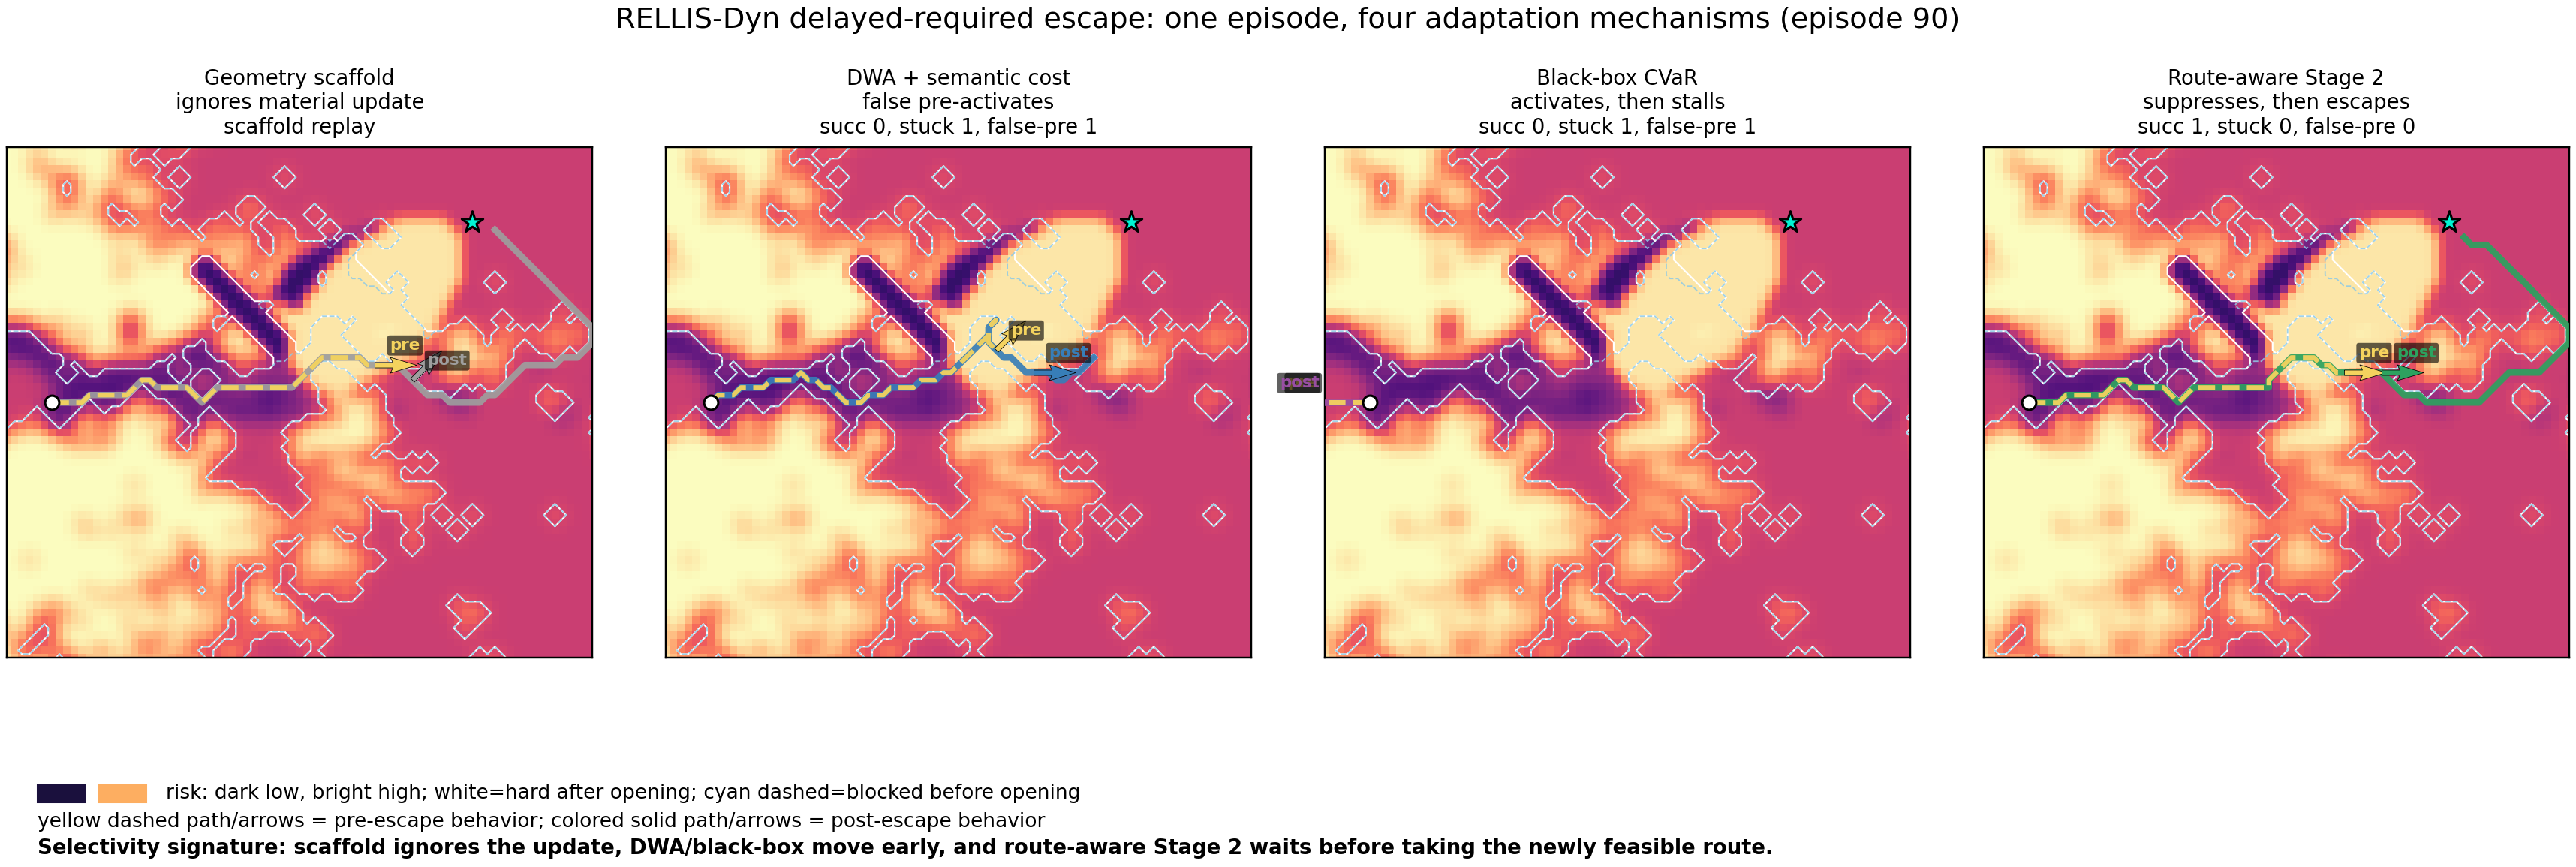
\includegraphics[width=\textwidth]{figures/rellis_dyn_spotlight_four_methods.png}
\caption{\textbf{Temporal selectivity in one delayed-required-escape episode.} Yellow dashed = behavior before the escape is available; solid colored = after it opens. Trajectories are \emph{measured rollouts}; no sampled witness primitive is drawn as an executed path. Geometry-only ignores the material update; DWA and black-box CVaR move before the escape is feasible and stall; the material-aware field suppresses before $t_{\rm escape}$ and takes the newly feasible route after.}
\label{fig:rellis_dyn_spotlight}
\end{figure*}

\paragraph{Interaction portability (highway).}
In highway-env, a lateral channel enables passing a slow leader while a time-to-collision channel suppresses it when the adjacent lane is boxed; only the full combination passes and suppresses correctly (App.~Table~\ref{tab:app_highway_mechanism}). MOBIL-IDM and risk-aware MPC lead overall, but the material-aware field is the strongest learned method and the only one showing the intended activation/suppression split.

\subsection{Limitations}
\label{sec:exp_limits}
(i) The hazard barrier $b_{\rm sp}(\phi)$ is differentiable but not a CBF certificate; violation numbers are empirical finite-rollout reductions (App.~\ref{app:theory}). (ii) Performance depends on risk-map quality; corruption degrades selectivity gradually (Table~\ref{tab:perception}), and the method uses no calibrated perception uncertainty. (iii) The gate is frame-wise and can flicker ($33.8\%$ single-step activations); temporal hysteresis is a natural extension. (iv) The method is weaker on moving-obstacle events where reactive boundary-following suffices. (v) Gate overhead should be profiled on latency-constrained hardware (ms/step, Table~\ref{tab:rellis_dyn_agg}).